\chapter{Revision}

\section{Pythagoras' Theorem}
For a right angle triangle with lengths $a$ and $b$, for hypotenuse $c$,
$c^2 = \sqrt{a^2 + b^2}$.

Proof:

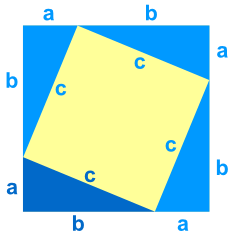
\includegraphics{img/pythagorean-theorem-proof.png}
\begin{align}
  \text{area}
    &= (a+b)^2 - 4(\frac{1}{2})ab \\
    &= a^2 + b^2 + 2ab - 2ab \\
    &= a^2 + b^2 \\
    &= c^2
\end{align}

This gives rise to \emph{irrational numbers}. Take a isosceles triangle of sides
1, 1, and $\sqrt{2}$.

%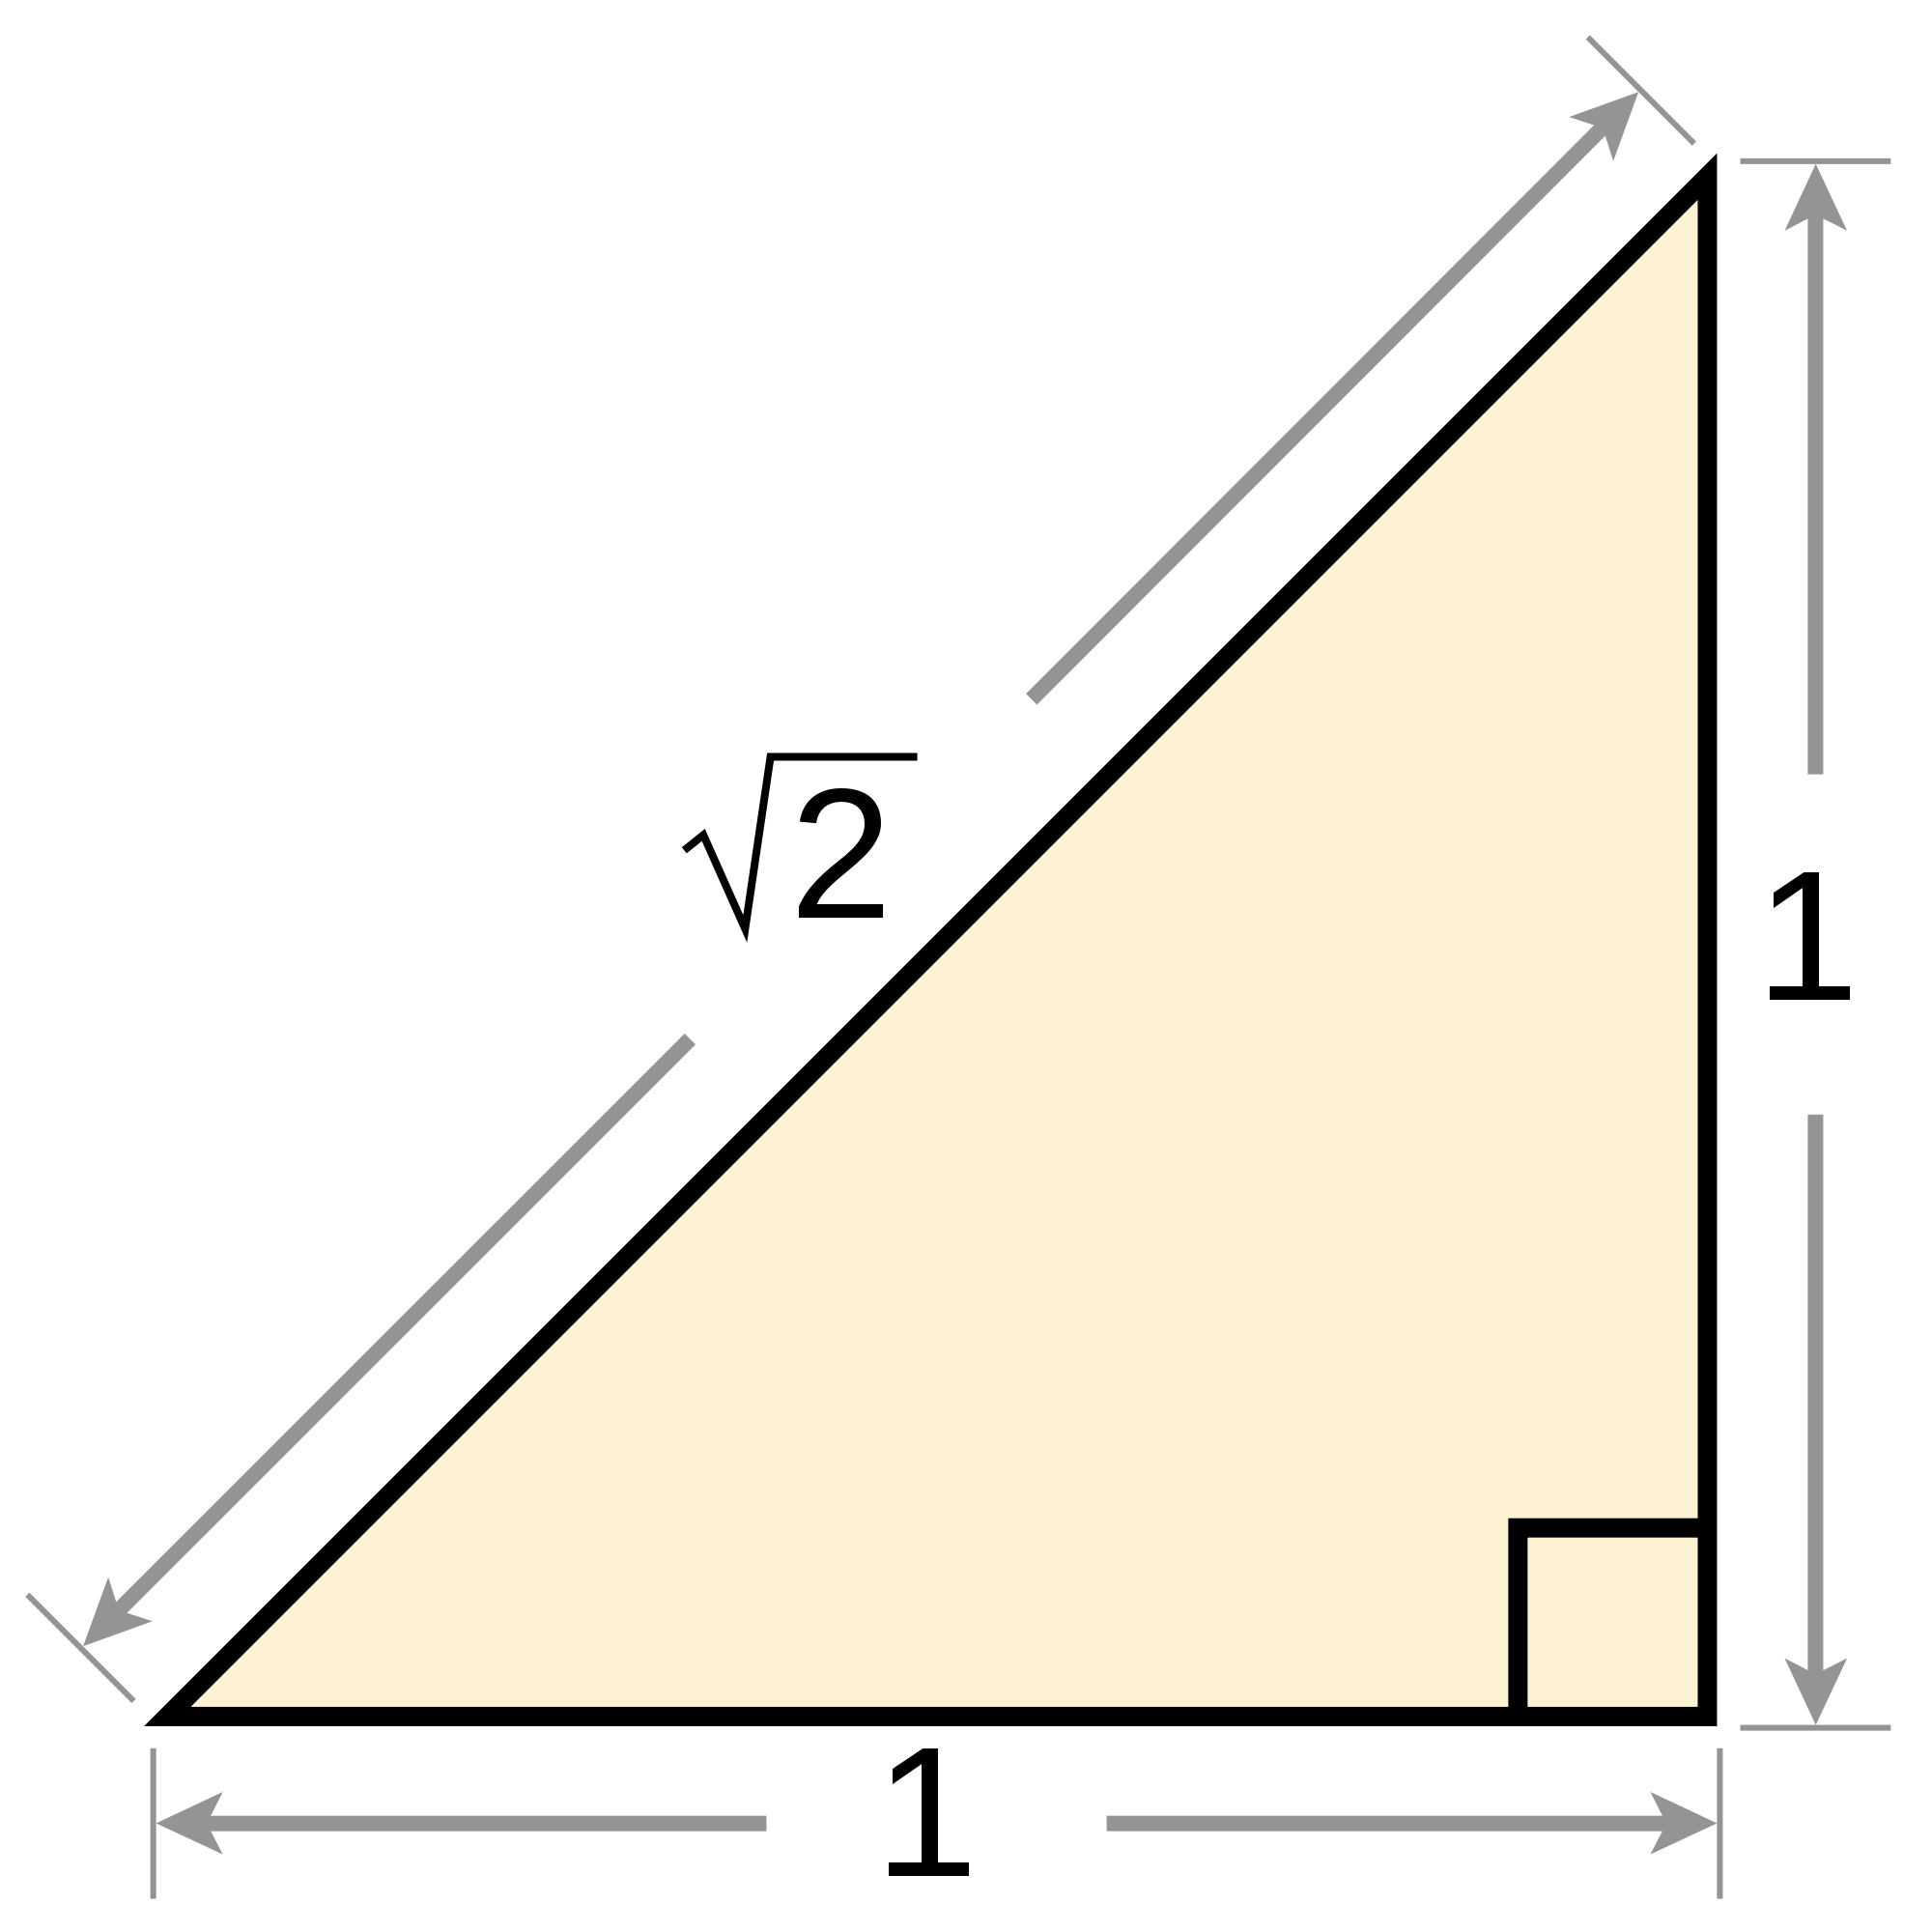
\includegraphics{img/2000px-Square_root_of_2_triangle.svg.png}
From this, we can deduce that $\sqrt{2}$ is not a fraction by using a proof by
contradiction.

For the moment, assume that $\sqrt{2}$ is rational:

\begin{align}
  \sqrt{2} &= \frac{p}{q} | p,q \in \mathbb{I} \text{and} q \neq 0 \\
  \text{Remove common factors from $p$ and $q$, that is assume}
  \gcd(p,q) &= 1
  \text{Hence}
  p &= q\sqrt{2} \\
    &= 2q^2
\end{align}

Lemma:

If $x$ is even, $x^2$ is even. \\
If $x$ is odd, $x^2$ is odd. \\
If $x = 2n \to x^2 = 4n$ is even. \\
If $x = 2n + 1 \to x^2 = 4n^2 + 4n + 1$ is an odd number.

Now $p^2$ is even, no $p$ is even, hence $p = 2m$ for some integer $m$. Then
\begin{align}
  p^2 &= 4m^2 & \\
      &= 2q^2 & \to q^2 = 2m^2 \text{even} \\
      &       & \to q \text{even}
\end{align}

So we have shown the assumption $\sqrt{2} = \frac{p}{q} \to p,q \text{even}$,
hence the assumption has to be false.


\section{Sets}
Most of modern mathematics is formulated on a domain of mathematics called
\emph{set theory}, a theory concerning a collection of objects.

\subsection{Examples of sets}
\begin{itemize}
  \item $\phi$ empty set with no elements
  \item $A = \{ 0, 1, 2, 3 \}$ a set of numbers from 0 to 3 inclusive called $A$.
  \item $0 := \phi$ zero is the empty set
  \item $1 := \{ 0 \}$
  \item $2 := \{ 0, 1 \}$
  \item $B = \{ x | \text{condition on x} \}$ define set based on condition
  \item $\mathbb{N} = \{ 0, 1, 2, ... \} $
  \item $\mathbb{Z} = \{ \text{ all integers} \}$
  \item $\mathbb{Q} = \{ \frac{p}{q} | p,q \in \mathbb{Z}, q \neq 0 \}$
  \item $\mathbb{R}$ real numbers
  \item $\mathbb{C}$ complex numbers
  \item We can define a set, $B$ in several ways:
  \begin{align}
    B &= \{ -2, -1, 0, 1, 2 \} \\
      &= \{ x \in \mathbb{Z} \quad | \quad -2 \leq x \leq 2 \} \\
      &= \{ x \in \mathbb{Z} \quad | \quad x^2 < 5 \}
  \end{align}
\end{itemize}

\subsection{Set Notation:}
\begin{itemize}
  \item $a \in \tilde{A}$ means "$a$ is in set of $\tilde{A}$"
  \item If $\tilde{A}$ and $\tilde{B}$ are sets, $\tilde{A} \subset \tilde{B}$
        means all elements of $\tilde{A}$ are in $\tilde{B}$.
  \item $a \notin \tilde{A}$ means "$a$ is not in set of $\tilde{A}$".
\end{itemize}

\subsection{Russell's Paradox}
Most sets are not elements of themselves.
\begin{align}
  A &= \{ 0, 1, 2, 3 \} \\
  A &\notin A
\end{align}


\begin{align}
  R &= \{ X | X \notin X \}
\end{align}

Question: Is $R$ a set?
If it is, then $R \in R$ iff $R \notin R$.

The solution is axiomatic: it required defining set theory. $R$ is not a set,
but is called a \emph{proper class}.

\section{Some other stuff in revision - common traps}
\begin{enumerate}
  \item $\sqrt{(-2)^2} = 2$ because square roots only yield positive numbers.
  \item $\sqrt{x^2} = |x|$
  \item $\sqrt{x}^2 = x$ because $x \geq 0$ in this case.
  \item $\int{\frac{1}{x}dx} = \log(x) + C^k$
  \item $\int_{-2}^{-1}{\frac{1}{x}dx} = \log|x| |_{-2}^{-1} = \log1 - \log2 = -\log2$ % TODO use evaluate symbol
\end{enumerate}

\section{Example of logarithmic function: Radioactive decay}
If at a certain time start with
% table
Time    Remaining amount
0       N(0)
$1t_{1/2}$ $N(0)/2$
$2t_{1/2}$ $N(0)/4)$
$3t_{1/2}$ $N(0)/8)$
... ...
\begin{align}
N(t) &= N(0) \cdot (\frac{1}{2})^{\frac{t}{t\frac{1}{2}}} \\
     &= N(0) \cdot e^{kt} \\
\text{where} \frac{1}{2} &= e^{\log{\frac{1}{2}}} \\
&= e^{-\log2} \text{st}
\text{with} k &= -\frac{\log2}{t\frac{1}{2}}
\end{align}

\section{Example in Radioactive (carbon) Dating}
Carbon comes in 3 different isotopes,  $^{12}_{6}$C (stable),
$^{13}_{6}$C (stable), $^{14}_{6}$C (radioactive). The half life
($t_\frac{1}{2}$) is 5730 years ($\pm 40$ years).

\begin{align}
  N(t) = N(0)\cdot(\frac{1}{2}^{\frac{t}{5730}}) | \text{where $t$ in years}
\end{align}

A skull has 15\% of the original $^{14}$C left. Estimate its age.

\begin{align}
  \frac{N(t)}{N(0)} &= 0.15 = (\frac{1}{2})^{\frac{t}{5730}} \\
  &= e^{-t(\frac{\log2}{5730})} \\
  \log(0.15) &= -t \frac{\log2}{5730} \\
  t &\approx 15683 \text{years}.
\end{align}

Always ask - does this result make sense? We know the half life is 5730, we have
50\% of the original C14 left. After 11000 years, it will be 25\%, and after
16000 years, it will be about 12.5\% left. 15\% is pretty close to 12.5\%, so
this answer makes sense.

...
